% Презентація до Завдання 2 (Хмарні обчислення): PDF -> Подкаст на Google Gemini API.
% Компіляція: xelatex / lualatex / pdflatex (двічі) або tectonic presentation.tex
% Також можна завантажити на Overleaf.
\documentclass[aspectratio=43]{beamer}

\usepackage{iftex}
\ifPDFTeX
  \usepackage[T2A]{fontenc}
  \usepackage[utf8]{inputenc}
  \usepackage{cmsrb}
\else
  \usepackage{fontspec}
  \setsansfont{cmunss.otf}[
    BoldFont=cmunsx.otf, ItalicFont=cmunsi.otf, BoldItalicFont=cmunso.otf]
  \setmonofont{cmuntt.otf}[
    BoldFont=cmuntb.otf, ItalicFont=cmunit.otf, BoldItalicFont=cmuntx.otf]
\fi
\usepackage[ukrainian]{babel}
\usepackage{booktabs}
\usepackage{array}
\usepackage{tikz}
\usetikzlibrary{positioning, arrows.meta, fit, backgrounds}

\usetheme{Madrid}
\setbeamertemplate{navigation symbols}{}
\setbeamertemplate{blocks}[rounded][shadow=true]

% Виділений тезис у сірому блоці, як у шаблоні
\newcommand{\thesis}[1]{\begin{block}{}#1\end{block}}

\title[PDF $\to$ Подкаст]{PDF $\to$ Подкаст}
\subtitle{Генерація подкастів з документів через Google Gemini API}
\author[І.С. Яценко]{Ілля Сергійович Яценко}
\institute[КНУТШ]{
  Кафедра теоретичної кібернетики \\
  Факультет комп'ютерних наук та кібернетики \\
  Київський національний університет імені Тараса Шевченка
}
\date{9 жовтня 2026 р.}

\begin{document}

\begin{frame}
  \titlepage
\end{frame}

% ------------------------------------------------------------------
\begin{frame}{Ідея}
  \thesis{Читати довгі статті важко, а слухати --- можна будь-де.}

  Статті, підручники, документація та звіти існують переважно як PDF.
  Їх неможливо «спожити» в транспорті, на прогулянці чи за кермом.

  \thesis{Перетворимо документ на \textbf{розмову двох ведучих}.}
  \begin{itemize}
    \item \textbf{Олена} --- ставить питання, які виникли б у слухача;
    \item \textbf{Віталій} --- пояснює зміст простими словами, з прикладами.
  \end{itemize}
  Діалог сприймається легше, ніж монотонне начитування тексту.
\end{frame}

% ------------------------------------------------------------------
\begin{frame}{Штучний інтелект як хмарний сервіс}
  \thesis{Хмара --- обчислювальні ресурси \textbf{за запитом} з
    \textbf{оплатою за використання}.}

  \small
  \begin{tabular}{@{}lll@{}}
    \toprule
    Модель & Що надає провайдер & Приклади \\
    \midrule
    IaaS & віртуальні машини, мережі, диски & Compute Engine, AWS EC2 \\
    PaaS & платформу для запуску коду & Cloud Run, Azure App Service \\
    SaaS & готовий застосунок & Gmail, Google Docs \\
    \textbf{AIaaS} & \textbf{готову AI-модель через API} & \textbf{Gemini API}, Azure OpenAI \\
    \bottomrule
  \end{tabular}
  \normalsize

  \thesis{Проєкт --- \textbf{споживач AIaaS}: ми не навчаємо й не
    розміщуємо модель, не купуємо GPU, а просто викликаємо її через API.}
\end{frame}

% ------------------------------------------------------------------
\begin{frame}{Хмарні платформи з AI-сервісами}
  \small
  \begin{tabular}{@{}lll@{}}
    \toprule
    Провайдер & Сервіс & Моделі \\
    \midrule
    Google Cloud & Gemini API, Vertex AI & Gemini, Imagen, Veo \\
    Microsoft Azure & Azure AI Foundry, AI Speech & GPT, Phi, Llama \\
    Amazon AWS & Amazon Bedrock, Polly & Claude, Nova, Llama \\
    \bottomrule
  \end{tabular}
  \normalsize

  \thesis{Обрано \textbf{Google Gemini API}.}
  \begin{itemize}
    \item і читання документа, і текст, і озвучення --- \textbf{в одному сервісі};
      в Azure чи AWS довелося б поєднувати кілька;
    \item модель сама читає PDF --- з текстом, таблицями й рисунками;
    \item безкоштовний рівень без банківської картки.
  \end{itemize}
\end{frame}

% ------------------------------------------------------------------
\begin{frame}{Gemini API}
  \thesis{Gemini --- сімейство моделей Google, що розуміють текст,
    зображення, аудіо, відео та PDF; за раз --- до \textbf{1 млн токенів}
    (ціла книга).}

  У проєкті використано дві моделі:
  \begin{itemize}
    \item \textbf{Gemini 3.8 Flash} --- читає документ і пише сценарій;
    \item \textbf{Gemini 3.8 Flash TTS} --- озвучує його двома голосами.
  \end{itemize}

  \begin{columns}[T]
    \begin{column}{0.48\textwidth}
      \thesis{\textbf{Gemini Developer API}}
      \small доступ за API-ключем, безкоштовний рівень --- для прототипів
      (використано в проєкті).
    \end{column}
    \begin{column}{0.48\textwidth}
      \thesis{\textbf{Vertex AI} (Google Cloud)}
      \small доступ через IAM, SLA, вибір регіону зберігання даних ---
      для промислового використання.
    \end{column}
  \end{columns}
\end{frame}

% ------------------------------------------------------------------
\begin{frame}{Як це працює: що в хмарі, а що локально}
  \centering
  \begin{tikzpicture}[
      box/.style={draw=structure, fill=structure!8, rounded corners,
        minimum width=2.4cm, minimum height=1.1cm, align=center, font=\small},
      api/.style={box, fill=structure, text=white},
      arr/.style={-{Stealth}, thick, structure},
      lbl/.style={font=\scriptsize, align=center}]
    \node[box] (user) {Користувач \\ \scriptsize браузер};
    \node[box, right=0.9cm of user] (srv) {Наш сервер \\ \scriptsize ноутбук, без GPU};
    \node[api, right=1.3cm of srv, yshift=0.8cm] (llm) {Gemini 3.8 Flash \\ \scriptsize сценарій};
    \node[api, below=0.5cm of llm] (tts) {Gemini TTS \\ \scriptsize озвучення};
    \begin{scope}[on background layer]
      \node[draw=structure, dashed, rounded corners, fill=structure!3, inner sep=8pt,
        fit=(llm)(tts), label={[font=\scriptsize, structure]above:Google Cloud}] {};
    \end{scope}
    \draw[arr] (user) -- node[lbl, above] {PDF} (srv);
    \draw[arr, {Stealth}-{Stealth}] (srv.east) -- ++(0.4,0) |- (llm.west);
    \draw[arr, {Stealth}-{Stealth}] (srv.east) -- ++(0.4,0) |- (tts.west);
    \draw[arr] (srv.south) -- ++(0,-0.6) -| node[lbl, pos=0.25, below] {MP3} (user.south);
  \end{tikzpicture}

  \vspace{0.8em}
  \raggedright
  \begin{columns}[T]
    \begin{column}{0.48\textwidth}
      \thesis{\textbf{У хмарі}}
      \small читання PDF, написання сценарію, синтез мовлення ---
      уся «важка» робота на GPU Google.
    \end{column}
    \begin{column}{0.48\textwidth}
      \thesis{\textbf{Локально}}
      \small інтерфейс, перевірка файлів, склеювання аудіо та
      збереження в MP3.
    \end{column}
  \end{columns}
\end{frame}

% ------------------------------------------------------------------
\begin{frame}{Веб-інтерфейс}
  \begin{columns}[c]
    \begin{column}{0.52\textwidth}
      \centering
      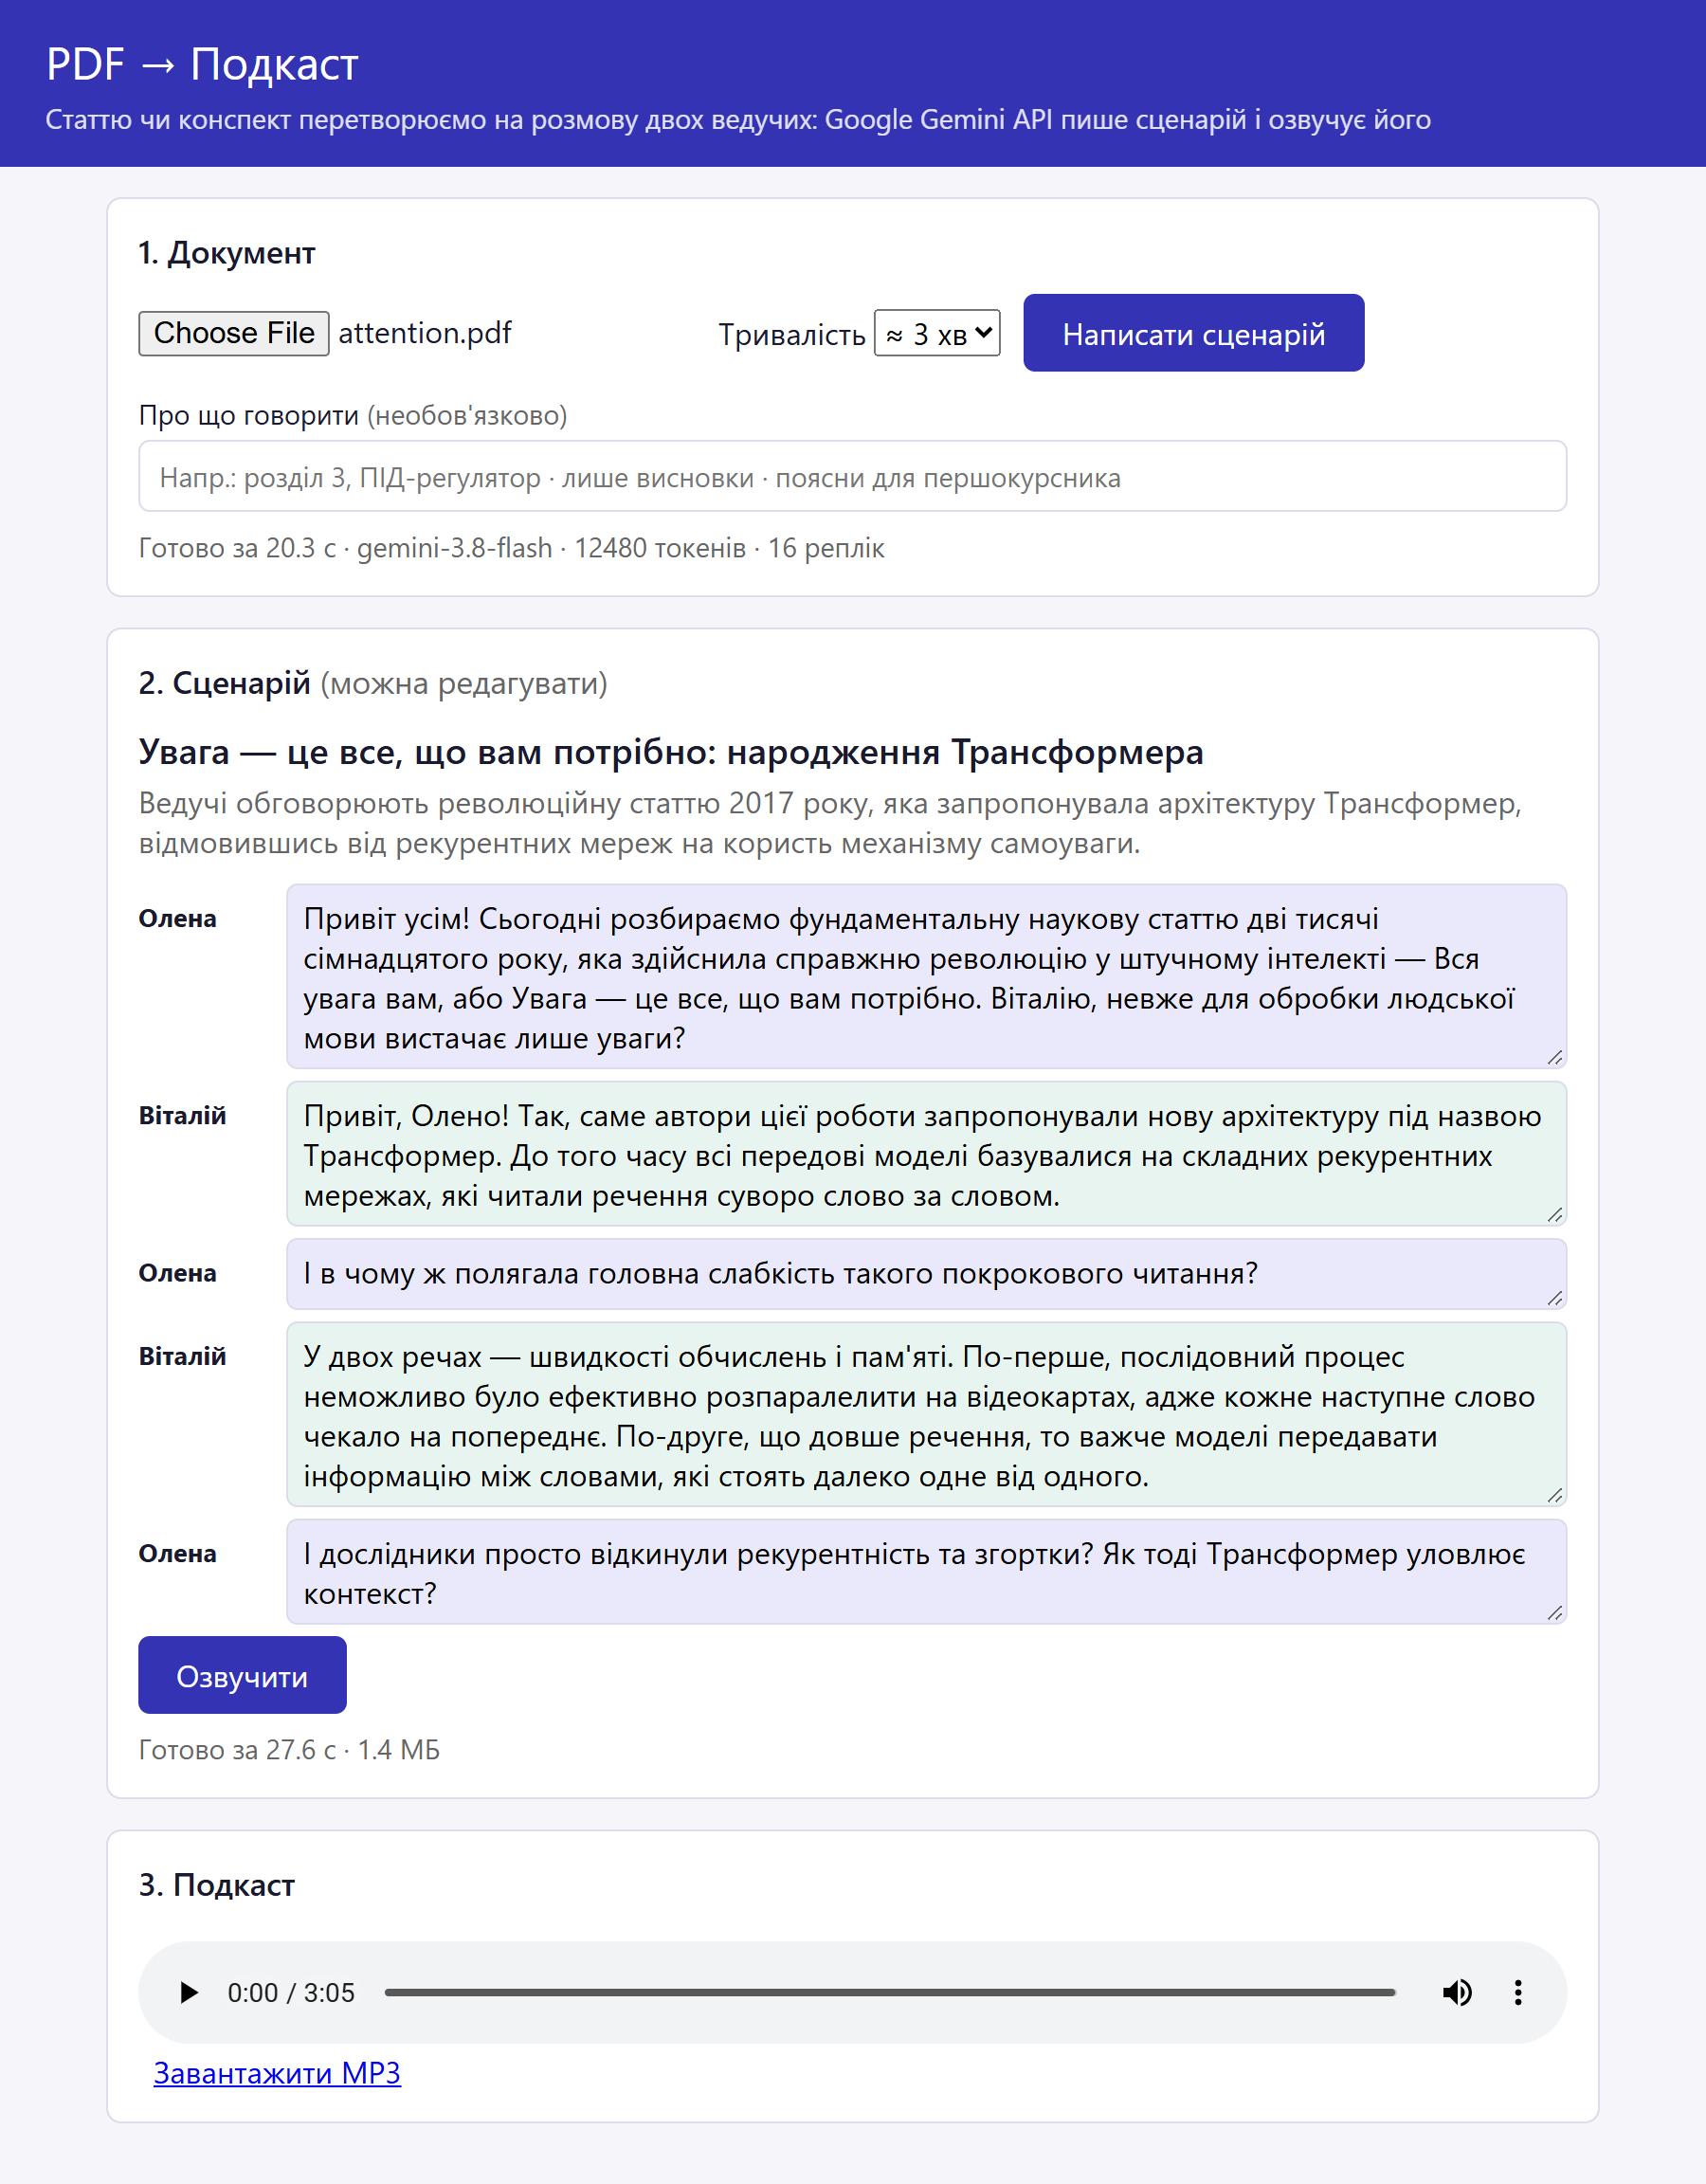
\includegraphics[width=\linewidth,height=0.86\textheight,keepaspectratio]{ui.png}
    \end{column}
    \begin{column}{0.44\textwidth}
      \begin{enumerate}\small
        \item Завантажити PDF, обрати тривалість і за бажанням --- тему.
        \item Переглянути сценарій і за потреби виправити репліки.
        \item Озвучити, прослухати й завантажити MP3.
      \end{enumerate}

      \thesis{\small Під кожним кроком --- скільки часу він зайняв.}
    \end{column}
  \end{columns}
\end{frame}

% ------------------------------------------------------------------
\begin{frame}{Що вміє програма}
  \begin{itemize}\small
    \item Перетворює PDF \textbf{будь-якою мовою} на подкаст \textbf{українською}.
    \item Двоє ведучих з \textbf{різними голосами й манерою}: жвава ведуча
      і спокійний експерт.
    \item Тривалість подкасту --- \textbf{від 1 до 10 хвилин}.
    \item \textbf{Фокус}: потрібний розділ великого документа («розділ 3»)
      або кут подачі («лише висновки», «для першокурсника»).
    \item \textbf{Редагування сценарію} перед озвученням.
    \item Результат --- \textbf{MP3}, зручний для телефона.
    \item Три способи роботи: \textbf{сайт}, командний рядок та
      \textbf{REST API} для вбудовування в інші системи.
    \item Якщо хмарна модель перевантажена --- \textbf{автоматично
      переходить на запасну}.
  \end{itemize}
\end{frame}

% ------------------------------------------------------------------
\begin{frame}{Чого програма не вміє}
  \begin{itemize}\small
    \item Озвучує \textbf{лише українською} та лише \textbf{двома голосами}
      з фіксованими іменами.
    \item Приймає \textbf{тільки PDF до 15 МБ} --- без Word, веб-сторінок
      чи відео.
    \item Формули, графіки й таблиці лише \textbf{переказує словами}.
    \item Може \textbf{спростити чи неточно передати} зміст --- сценарій
      варто перевіряти.
    \item Працює \textbf{не миттєво}: близько хвилини на подкаст.
    \item \textbf{Без інтернету не працює} --- уся генерація в хмарі.
    \item Це \textbf{прототип}: запускається локально, без акаунтів та
      історії подкастів.
  \end{itemize}

  \thesis{Більшість обмежень --- свідомі спрощення прототипу, а не
    обмеження хмарного сервісу.}
\end{frame}

% ------------------------------------------------------------------
% Справжній результат: examples/attention.json, examples/attention.mp3
\begin{frame}{Приклад: «Attention Is All You Need»}
  \textbf{Вхід:} наукова стаття, з якої почалися сучасні мовні моделі
  (15 сторінок, англійською).

  \vspace{0.5em}
  \textbf{Вихід:} подкаст українською «Увага --- це все, що вам потрібно:
  народження Трансформера».
  \begin{itemize}\small
    \item[] \textbf{Олена:} \emph{Але якщо всі слова аналізуються одночасно,
      як Трансформер розуміє їхній порядок?}
    \item[] \textbf{Віталій:} \emph{Для цього застосували позиційне кодування.
      До векторів слів додали спеціальні числові мітки…}
  \end{itemize}

  \small
  \begin{tabular}{@{}ll@{\qquad}ll@{}}
    сценарій: & 16 реплік, 20 с & озвучення: & 28 с \\
    аудіо: & 3 хв 05 с, 1,4 МБ & вартість: & 0 на безкоштовному рівні \\
  \end{tabular}
  \normalsize

  \thesis{Переклад, спрощення та озвучення --- менше ніж за хвилину.}
\end{frame}

% ------------------------------------------------------------------
\begin{frame}{Скільки це коштує}
  \thesis{Хмарна модель оплати \textbf{pay-as-you-go}: платимо лише за
    оброблені \textbf{токени} --- без серверів і підписок.}

  \small
  \begin{tabular}{@{}>{\raggedright}p{0.16\textwidth}>{\raggedright}p{0.38\textwidth}
                    >{\raggedright\arraybackslash}p{0.38\textwidth}@{}}
    \toprule
    & \textbf{Безкоштовний рівень} & \textbf{Платний рівень} \\
    \midrule
    Ціна & 0 & $\sim$кілька центів за подкаст (оцінка) \\
    Ліміти & обмежена кількість запитів на хвилину й добу & вищі \\
    Дані & можуть використовуватися для покращення продуктів Google &
      не використовуються \\
    \bottomrule
  \end{tabular}
  \normalsize

  \vspace{0.5em}
  \begin{itemize}\small
    \item Для навчання й демонстрації безкоштовного рівня достатньо.
    \item Хмарні ціни змінюються: тарифи Gemini 3.8 подвояться з 1 січня 2027.
  \end{itemize}
\end{frame}

% ------------------------------------------------------------------
\begin{frame}{Сфери застосування}
  \begin{columns}[T]
    \begin{column}{0.5\textwidth}
      \begin{itemize}\small
        \item \textbf{Освіта}: підручники та лекції в аудіоформаті;
        \item \textbf{Доступність}: для людей з вадами зору чи дислексією;
        \item \textbf{Наука}: огляди нових статей «на ходу»;
        \item \textbf{Мовне навчання}: діалоги за текстом іноземною мовою;
      \end{itemize}
    \end{column}
    \begin{column}{0.5\textwidth}
      \begin{itemize}\small
        \item \textbf{Бізнес}: звіти та регламенти для співробітників;
        \item \textbf{Онбординг}: документація у форматі розмови;
        \item \textbf{Медіа}: подкасти з блогів і новин;
        \item \textbf{Маркетинг}: аудіоверсії white paper.
      \end{itemize}
    \end{column}
  \end{columns}

  \vspace{0.5em}
  \thesis{Схожа функція є в Google NotebookLM --- наш прототип відтворює
    її через публічний API, тож її можна вбудувати у власний продукт.}
\end{frame}

% ------------------------------------------------------------------
\begin{frame}{Як розвинути проєкт у хмарі}
  \begin{itemize}
    \item \textbf{Cloud Run} (PaaS) --- розгорнути сервер у хмарі: доступ з
      будь-якого пристрою й автоматичне масштабування.
    \item \textbf{Cloud Storage} --- зберігати подкасти й ділитися посиланням.
    \item \textbf{Pub/Sub} або \textbf{Cloud Tasks} --- черга завдань для
      великих документів, щоб не чекати на сторінці.
    \item \textbf{Firebase Authentication} --- акаунти та історія подкастів.
    \item \textbf{Vertex AI} --- для конфіденційних документів: вибір регіону
      й гарантії щодо даних.
  \end{itemize}

  \thesis{Кожен крок --- ще один хмарний сервіс, а не власна інфраструктура.}
\end{frame}

% ------------------------------------------------------------------
\begin{frame}{Висновки}
  \begin{enumerate}
    \item Хмарний AI-сервіс дав змогу створити продукт \textbf{без власних
      моделей і GPU} --- уся «важка» робота виконується в Google Cloud.
    \item Програма перетворює PDF на подкаст українською \textbf{менше ніж
      за хвилину}, з фокусом на потрібній темі та можливістю редагування.
    \item Модель оплати \textbf{pay-as-you-go}: прототип --- безкоштовно,
      масштабування --- центи за подкаст.
  \end{enumerate}

  \thesis{Код проєкту: \url{https://github.com/ilyayath/pdf-to-podcast}}
\end{frame}

% ------------------------------------------------------------------
\begin{frame}
  \centering
  \vfill
  {\Huge Дякую за увагу!}
  \vfill
\end{frame}

\end{document}
